\subsubsection{Servizi}

\paragraph{AuthenicationService} \label{AuthenticationService}
\begin{figure}[H]
    \centering
    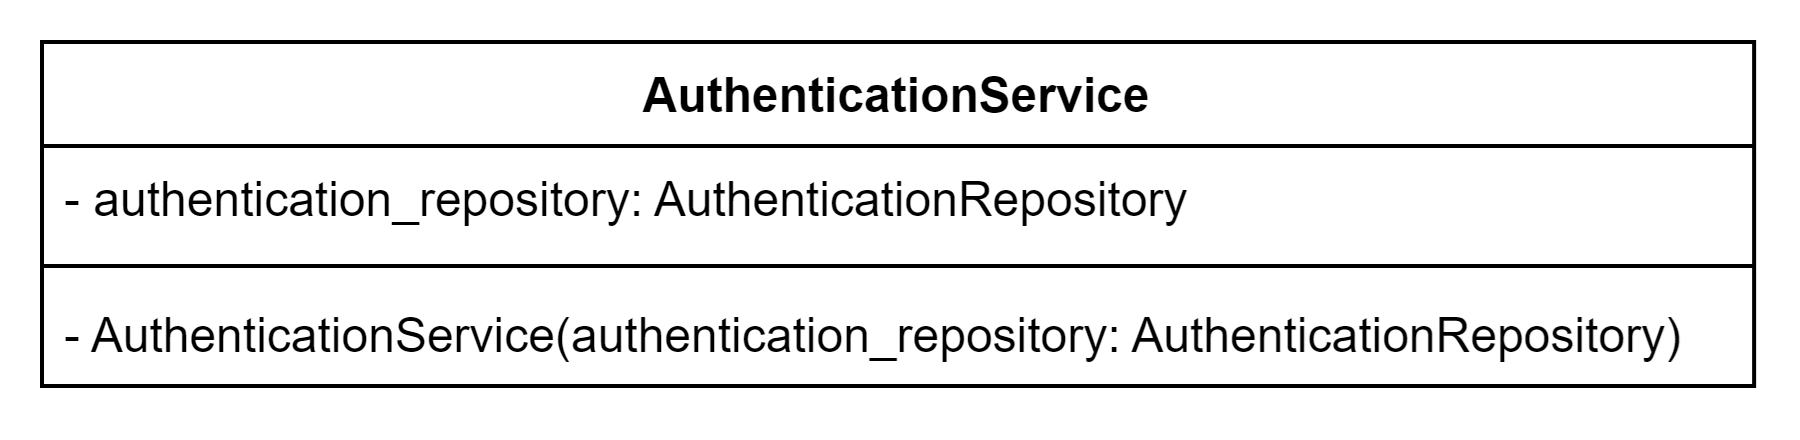
\includegraphics[width=0.95\textwidth]{assets/Backend/authentication_service.png}
    \caption{Rappresentazione della classe AuthenticationService}
  \end{figure}
\begin{itemize}
    \item \textbf{Descrizione:} Questa classe si occupa di gestire l'autenticazione degli utenti.
    \item \textbf{Implementazione:} Questa classe implementa la porta \texttt{AuthenticationUseCase}.
    \item \textbf{Attributi:}
    \begin{itemize}
        \item \texttt{authentication\_repository: AuthenticationRepository}: la \glossario{repository} usata per il recupero dei dati.
    \end{itemize}
    \item \textbf{Metodi:}
    \begin{itemize}
        \item \texttt{+ login(username: string, password: string): AuthResponseDto}: conferma un utente con username e password. Ritorna un oggetto di risposta, contenente il risultato dell'autenticazione.
    \end{itemize}
    \item \textbf{Dipendenze:}
    \begin{itemize}
        \item \texttt{AuthenticationUseCase}
        \item \texttt{AuthenticationRepository}
    \end{itemize}
\end{itemize}  

\paragraph{DictionaryService} \label{DictionaryService}
\begin{figure}[H]
    \centering
    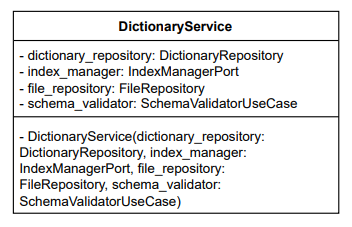
\includegraphics[width=0.95\textwidth]{assets/Backend/dictionary_service.png}
    \caption{Rappresentazione della classe DictionaryService}
  \end{figure}
\begin{itemize}
    \item \textbf{Descrizione:} questa classe si occupa di gestire le operazioni sul \glossario{dizionario dati}. 
    \item \textbf{Implementazione:} questa classe implementa la porta \texttt{DictionaryUseCase}. 
    \item \textbf{Attributi:}
    \begin{itemize}
        \item \texttt{dictionary\_repository: DictionaryRepository}: la repository usata per il recupero dei dati;
        \item \texttt{index\_manager: IndexManagerPort}: gestore dell'indicizzazione e del recupero dei dati;
        \item \texttt{file\_repository}: la repository usata per le operazioni sul file;
        \item \texttt{schema\_validator: SchemaValidatorUseCase}: il validatore degli schemi per il dizionario dati.
    \end{itemize}
    \item \textbf{Metodi:}
    \begin{itemize}
        \item \texttt{+ get\_dictionary\_list(): DicionariesResponseDto}: recupera la lista di tutti i dizionari;
        \item \texttt{+ get\_dictionary\_by\_id(id: integer): Union[DictionaryResponseDto, ResponseDto]}: recupera un dizionario tramite il suo id;
        \item \texttt{+ get\_dictionary\_file(id: integer): Optional[string]}: recupera il contenuto del file del dizionario dato il suo id;
        \item \texttt{+ get\_dictionary\_preview(id: integer): DictionaryResponseDto}: recupera l'anteprima del dizionario, dato il suo id;
        \item \texttt{+ create\_dictionary(dictionary: DictionaryDto, content: string): DictionaryResponseDto}: crea un nuovo dizionario e salva il suo file;
        \item \texttt{+ update\_dictionary\_metadata(id: integer, dictionary: DictionaryDto): DictionaryResponseDto}: aggiorna i metadati di un dizionario esistente;
        \item \texttt{+ update\_dictionary\_file(id: integer, content: string): DictionaryResponseDto}: aggiorna il contenuto del file di un dizionario esistente;
        \item \texttt{+ delete\_dictionary(id: integer): ResponseDto}: elimina un dizionario esistente, i suoi file associati e il suo indice.
    \end{itemize}
    \item \textbf{Dipendenze:}
    \begin{itemize}
        \item \texttt{DictionaryUseCase}
        \item \texttt{DictionaryRepository}
        \item \texttt{IndexManagerPort}
        \item \texttt{FileRepository}
        \item \texttt{SchemaValidatorUseCase}
    \end{itemize}
\end{itemize}

\paragraph{PromptManagerService} \label{PromptManagementService}
\begin{figure}[H]
    \centering
    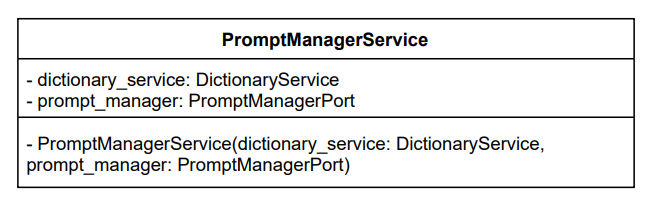
\includegraphics[width=0.95\textwidth]{assets/Backend/prompt_manager_service.png}
    \caption{Rappresentazione della classe PromptManagerService}
  \end{figure}
\begin{itemize}
    \item \textbf{Descrizione:} questa classe si occupa di gestire le operazioni per la generazione dei \glossario{prompt}.
    \item \textbf{Implementazione:} questa classe implementa la porta \texttt{PromptUseCase}. 
    \item \textbf{Attributi:}
    \begin{itemize}
        \item \texttt{dictionary\_service: DictionaryService}: il servizio per la gestione dei \glossario{dizionario dati};
        \item \texttt{prompt\_manager: PromptManagerPort}: il gestore della generazione dei prompt;
    \end{itemize}
    \item \textbf{Metodi:}
    \begin{itemize}
        \item \texttt{+ generate\_prompt(dictionary\_id: integer, query: string, dbms: string, language: string): StringDataResponseDto}: genera un prompt per un dizionario dato il suo id, la richiesta inserita, il dbms e la lingua selezionati;
        \item \texttt{+ generate\_prompt\_with\_debug(dictionary\_id: integer, query: string, dbms: string, language: string): PromptResponseDto}: genera un prompt con le informazioni di \glossario{debug};
        \item \texttt{- generate\_prompt(dictionary\_id: integer, query: string, dbms: string, language: string, log: bool): tuple}: metodo interno per la generazione del prompt usando il prompt manager.
    \end{itemize}
    \item \textbf{Dipendenze:}
    \begin{itemize}
        \item \texttt{PromptUseCase}
        \item \texttt{DictionaryService}
        \item \texttt{PromptManagerPort}
    \end{itemize}
\end{itemize}  